% Copyright 2024 Kieran W Harvie. All rights reserved.
\documentclass[12pt]{report}

% Copyright 2023 Kieran W Harvie. All rights reserved.
\usepackage{amsmath}
\usepackage{titlesec}
\usepackage{hyperref}
\usepackage{amssymb}
\usepackage{tikz}
 
\usepackage[OT2,T1]{fontenc}

\titleformat{\chapter}[display]
	{\normalfont\huge\bfseries}{}{0pt}{\Huge}
\titlespacing*{\chapter}
	{0pt}{10pt}{40pt}

\DeclareSymbolFont{cyrletters}{OT2}{wncyr}{m}{n}

\DeclareMathOperator{\sinc}{sinc}
\DeclareMathOperator{\Ai}{Ai}
\DeclareMathSymbol{\Sha}{\mathalpha}{cyrletters}{"58}
\DeclareMathOperator{\Hom}{Hom}
\DeclareMathOperator{\cl}{cl}
\DeclareMathOperator{\im}{Im}
\DeclareMathOperator{\rect}{rect}
\DeclareMathOperator{\sgn}{sgn}
\DeclareMathOperator{\XOR}{ XOR }
\DeclareMathOperator{\E}{\mathbb{E}}
\DeclareMathOperator{\img}{img}
\DeclareMathOperator{\ord}{ord}
\DeclareMathOperator{\Res}{Res}


\hypersetup{
	pdftitle = {Blossom Theory},
	pdfpagemode = {UseOutlines},
	pdfauthor = {Kieran Harvie},
	pdfsubject = {Blossom Theory, Bézier Curves and Surfaces, CAD},
	pdfkeywords = {TODO},
	pdfborder =  {2 2 1},
}

\usepackage{biblatex}
\addbibresource{blossom_theory.bib}

\title{Blossom Theory\\ \large An Intuitive and Practical Foundation for Bézier Curves and Surfaces}
\date{Copyright \textcopyright\,  \today. All Rights Reserved.}
\author{Kieran Harvie}

\renewcommand\thechapter{}
\renewcommand\thesection{\arabic{section}}

\begin{document}
\maketitle

% Copyright 2024 Kieran W Harvie. All rights reserved.

\topskip0pt
\vspace*{\fill}
\begin{center}
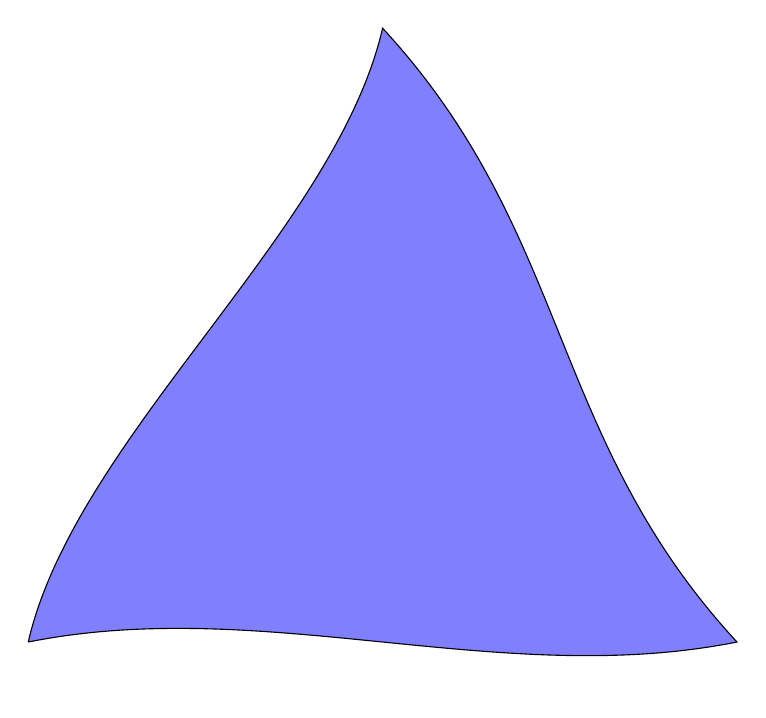
\begin{tikzpicture}[scale=1.5,every node/.style={black}]
%	\coordinate (    ) at (Y+Z*2    , Y*1.7320508075    );
	\coordinate (p300) at (0+0*2    , 0*1.7320508075    );
	\coordinate (p210) at (1+0*2-0.6, 1*1.7320508075    );
	\coordinate (p201) at (0+1*2    , 0*1.7320508075+0.4);
	\coordinate (p120) at (2+0*2+0.6, 2*1.7320508075    );
	\coordinate (p111) at (1+1*2    , 1*1.7320508075    );
	\coordinate (p102) at (0+2*2    , 0*1.7320508075-0.4);
	\coordinate (p030) at (3+0*2    , 3*1.7320508075    );
	\coordinate (p021) at (2+1*2+0.6, 2*1.7320508075    );
	\coordinate (p012) at (1+2*2-0.6, 1*1.7320508075    );
	\coordinate (p003) at (0+3*2    , 0*1.7320508075    );
	\coordinate (p300) at (0+0*2    , 0*1.7320508075    );

	\filldraw[fill=blue!50] (p300) .. controls (p210) and (p120) ..  (p030) .. controls (p021) and (p012) .. (p003) .. controls (p102) and (p201) .. (p300);
\end{tikzpicture}

An example Cubic Bézier Triangle rendered natively and easily within this very \LaTeX document.
\end{center}
\vspace*{\fill}

\newpage

% Copyright 2024 Kieran W Harvie. All rights reserved.

\section{Introduction}
Bézier curves and surfaces are an elegant way to enhance our models and renders with natural curves.
The foremost resource on the application of curves and surfaces to these problems,
the resource that many an intrigued person is pointed to,
is "Curves and Surfaces for CAGD"\cite{CAGD}.
This work is phenomenal.
Providing a wonderful treatment on not only Bézier curves and surfaces but surrounding theory of blossoms,
the algorithm poetically call "the blossoming",
and along with other more general curves and surfaces.
I can't understate how much anyone reading this document would find value in reading it too.
\\

However,
while reading the book,
I was continuously compelled to rewrite the presented mathematics in a style more familiar to me,
this document is the end result of that compulsion.
This style,
along with targeted level of audience knowledge,
is the esteemed undergraduate textbook "Algebra" by Artin\cite{artin}.
The results needed from Artin are nothing more complex than knowing what an $R$-module is or why every vector space has basis.
Additionally any background material outside of Artin has been included in the appendix,
A choice Artin made himself.
\\

This book will begin by describing various Bézier curves and surfaces along with the properties Bernstein basis polynomials
under the general umbrella of `Bézier Geometry'.
The we will define Blossoms and the blossoming.
Finally we will combine the two and apply blossoms too Bézier Geometry.


\chapter{Bézier Geometry}
% Copyright 2024 Kieran W Harvie. All rights reserved.

\section{Bernstein Basis Polynomials}
The $k^\text{th}$ Bernstein basis polynomial of order $n$ is defined as:
\[
	b_{k,n}(t) = \binom{n}{k}(1-t)^{n-k}t^k
\]
Where we follow that convention that $\binom{n}{k}=0$ when $k<0$ or $k>n$.
\\

They have some really useful properties that lend them themselves to applications like
approximating continuous functions,
numerically stable polynomial evaluation, 
and are the foundation of Bézier geometry.
To this end it will be useful to collect some of those properties bellow.
\begin{center}
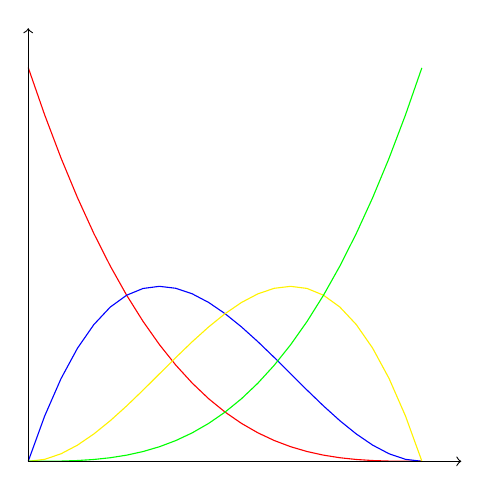
\begin{tikzpicture}[domain=0:1,scale=5]
	\draw[red] plot (\x,{(1-\x)^3});
	\draw[blue] plot(\x,{3*\x*(1-\x)^2});
	\draw[yellow] plot (\x,{3*\x*\x*(1-\x)});
	\draw[green] plot (\x,{\x*\x*\x});

	\draw[<->] (0,1.1)--(0,0)--(1.1,0);
\end{tikzpicture}

The four Bernstein basis polynomials of degree three over $[0,1]$.
\end{center}

\subsubsection{Fundamental Recursion:}
The most fundamental property of Bernstein basis polynomials is the recursion:
\[b_{k,n+1}(t) = (1-t)b_{k,n}(t)+tb_{k-1,n}(t)\]
And that there are $n+1$ polynomials of order $n$,
since when $k<0$ or $k>n$ we have:
\[b_{k,n}(t) = 0\]
Both of these properties can be verified by inspection of the definition and let us create a table of low order Bernstein basis polynomials to further cultivate intuition:
\[
\begin{array}{|c|ccccc|}
	\hline
	b_{k,n}(t)&0&1&2&3&4\\
	\hline
	4&(1-t)^4&4t(1-t)^3&6t^2(1-t)^2&4t^3(1-t)&t^4\\
	3&(1-t)^3&3t(1-t)^2&3t^2(1-t)&t^3&\\
	2&(1-t)^2&2t(1-t)&t^2&&\\
	1&1-t&t&&&\\
	0&1&&&&\\
	\hline
\end{array}
\]

\subsubsection{Endpoints:}
In most application we will be considering $t\in[0,1]$.
So it makes sense to consider $b_{k,n}(0)$ and $b_{k,n}(1)$ as the `endpoints' and note  their values as:
\[b_{k,n}(0) = \begin{cases}1& k=0\\0&k\neq0\\\end{cases}\quad\text{and}\quad b_{k,n}(1) = \begin{cases}1& k= n\\0&k\neq n\\\end{cases}\]

\subsubsection{Product:}
The product of two Bernstein basis polynomials is another one:
\[\begin{aligned}
	b_{k,n}(t)b_{l,m}(t) =& \binom{n+m}{k+l}^{-1}\binom{n}{k}\binom{m}{l}b_{k+l,n+m}(t)\\
	=&\binom{n+m}{m}^{-1}\binom{k+l}{l}\binom{n+m-(k+l)}{m-l}b_{k+l,n+m}(t)\\
\end{aligned}\]

\subsubsection{Inner Product and Partition of Unity:}
The following combinatorial identity can be verified by expansion:
\[\binom{n}{l}\binom{l}{k} = \binom{n}{k}\binom{n-k}{l-k}\]
When combined with the binomial theorem it allows us evaluate an `inner product' of Bernstein basis polynomials:
\[\begin{aligned}
	\sum_{l=k}^nb_{k,l}(t)b_{l,n}(\tau) =& \sum_{l=k}^n\binom{n}{l}\binom{l}{k}t^l\tau^k(1-t)^{n-l}(1-\tau)^{l-k}\\
	=& \binom{n}{k}(t\tau)^k\sum_{l=k}^n\binom{n-k}{l-k}(1-t)^{n-l}(t(1-\tau))^{l-k}\\
	=& \binom{n}{k}(t\tau)^k\sum_{l=0}^{n-k}\binom{n-k}{l}(1-t)^{n-l-k}(t(1-\tau))^{l}\\
	=& \binom{n}{k}(t\tau)^k(1-t+t(1-\tau))^{n-k}\\
	=& b_{k,n}(t\tau)\\
\end{aligned}\]
In particular,
when $k$ and $\tau$ equal $0$, we have:
\[b_{k,l}(\tau) = b_{k,n}(t\tau) = 1\]
Which substitution into the general case gives:
\[\sum_{l=0}^nb_{l,n}(t) = 1\]
Hence,
for any given $n$,
the polynomials $b_{k,n}(t)$ are a partition of unity.

\subsubsection{Reflection:}
From the following binomial formula:
\[\binom{n}{k}=\binom{n}{n-k}\]
We get the following formula for reflecting argument around $\frac{1}{2}$:
\[b_{k,n}(t) = b_{n-k,n}(1-t)\]
Which gives my favourite Bernstein basis polynomial formula: 
\[ b_{k,m}(\tau+(1-\tau)t) = \sum_{l=0}^kb_{k-l,n-l}(\tau)b_{l,n}(t) \]
By applying the reflection to the inner product formula:
\[\begin{aligned}
	b_{k,n}(\tau+(1-\tau)t) =& b_{k,n}(1-(1-t)(1-\tau))\\
	=& b_{n-k,n}((1-t)(1-\tau))\\
	=&\sum_{l=n-k}^nb_{n-k,l}(1-\tau)b_{l,n}(1-t)\\
	=&\sum_{l=n-k}^nb_{k-(n-l),l}(\tau)b_{n-l,n}(t)\\
\end{aligned}\]
And then change the summation order so $l$ goes down from $n$ instead of up from $n-k$.

\subsubsection{Bounds:}
When $t\in[0,1]$ we have both $t\geq0$ and $1-t\geq0$ and hence:
\[t\in [0,1] \Rightarrow b_{k,n}(t)\geq0 \]
Now since each individual polynomial is positive we have:
\[b_{k,n}(t) \leq \sum_{k=0}^nb_{k,n}(t) = 1\]

\subsubsection{Derivative:}
By direct application of the product rule we get:
\[b_{k,n+1}'(t) = k\binom{n+1}{k}(1-t)^{n+1-k}t^{k-1}-(n+1-k)\binom{n+1}{k}(1-t)^{n-k}t^k\]
Simpling the coefficients containing $k$ into the binomial coefficients we obtain:
\[b_{k,n+1}'(t) = (n+1)(b_{k-1,n}(t)-b_{k,n}(t))\]
If we instead factor common terms we get:
\[b_{k,n+1}'(t) = (1-t)^{n-k}t^{k-1}\binom{n+1}{k}\bigg(k(1-t)-(n+1-k)t\bigg)\]
When $t\in(0,1)$ the first three factors are non-negative,
hence there can only be an extrema where the fourth factor is zero at $t=\frac{k}{n+1}$.
By considering the endpoints this extrema must be a maximum and is the only extrema on $t\in[0,1]$.

\subsubsection{Useful Sums:}
We have already used binomial expansion when calculating the inner product.
However, if we consider the general expression:
\[(x+y)^n = \sum_{k=0}^n\binom{n}{k}x^{n-k}y^k\]	
When derived by $y$:
\[n(x+y)^{n-1} = \sum_{k=0}^nk\binom{n}{k}x^{n-k}y^{k-1}\]
Multiplied by $y(x+y)$:
\[ny(x+y)^n = (x+y)\sum_{k=0}^nk\binom{n}{k}x^{n-k}y^k\]
And having set $x=1-t$ and $y=t$:
\[nt = \sum_{k=0}^nk\binom{n}{k}(1-t)^{n-k}t^k\ = \sum_{k=0}^nkb_{k,n}(t)\]
We get this sum with simple terms.
The simplicity makes it a useful starting point and sanity check when writing algorithms involving the Bernstein basis polynomials.
For example,
if we are writing an algorithm for calculating the value of a Bernstein basis expansion at $t$ we know that if we choose linearly increasing coefficients we should get a linear function of $t$.
If we conversely want the Bernstein basis expansion of a linear function we know to use linearly increasing coefficients.	
\\

Through similar methods we get similar sums for higher powers, for example:
\[n(n-1)t^2 = \sum_{k=0}^nk(k-1)b_{k,n}(t)\]
They are useful for similar starting points and sanity checks for derivatives.
For example if we choose quadratically increasing coefficients in a Bernstein basis expansion we should get a linear derivative.

% Copyright 2024 Kieran W Harvie. All rights reserved.

\section{Bézier Curves}
Given $n+1$ control points $\mathbf{P}_k$ the $n$th order Bézier curve is given by:
\[
	f(t) = \sum_{k=0}^nb_{k,n}(t)\mathbf{P}_k,\quad t\in [0,1]
\]
Note that sometimes the function itself,
without the domain,
is also called a Bézier curve.
\\

The lower order Bézier curves have their expected special names,
for example a Linear Bézier curve is:
\[f(t)=(1-t)\mathbf{P}_0+t\mathbf{P}_1\]
A Quadratic Bézier curve is:
\[f(t)=(1-t)^2\mathbf{P}_0+2t(1-t)\mathbf{P}_1+t^2\mathbf{P}_2\]
And a Cubic Bézier curve is:
\[f(t)=(1-t)^3\mathbf{P}_0+3t(1-t)^2\mathbf{P}_1+3t^2(1-t)\mathbf{P}_2+t^3\mathbf{P}_3\]
These curves are the most common ones you will see in practice,
Cubic Bézier curves in particular,
as it has wide support across many programs.

\begin{center}
\begin{tikzpicture}
	\draw[red] (0,0) .. controls (1,3) and (4,0) .. (5,3);
	\filldraw (0,0) node[above]{} circle(2pt);
	\filldraw (1,3) node[above]{} circle(2pt);
	\filldraw (4,0) node[above]{} circle(2pt);
	\filldraw (5,3) node[above]{} circle(2pt);
\end{tikzpicture}

An example Cubic Bézier curve with control points shown.
\end{center}

\subsubsection{Interpreting the control points}
There's two interpretations on the control points of a Bézier curve.
\\

First is that the points determine the location and derivatives of the start and end points.
The curve starts at $\mathbf{P}_0$ and ends at $\mathbf{P}_n$.
Its derivative at the start lies on $\mathbf{P}_1-\mathbf{P}_0$ and at the end on $\mathbf{P}_{n-1}-\mathbf{P}_n$.
Its second derivative at the start is controlled by $\mathbf{P}_2$ and end by $\mathbf{P}_{n-2}$, etc.
A corollary of this is that two curves who share all their control points less than $k$ have the same $k$ or less derivatives at the start of the curves,
likewise for $k$ and above and $n-k$ and the curves end.
\\

Second is that the points pull the curve towards them and with a strength and variability determined by $b_{k,n}$.
To see this let $f$ and $\hat{f}$ be $n$ Bézier Curves that differ only with control point $\mathbf{P}_k$ and $\hat{\mathbf{P}_k}$, then we have.
\[
	\hat{f}(t) = b_{k,n}(t)(\hat{\mathbf{P}}_k-\mathbf{P}_k)+f(t)
\]
Since $b_{k,n}$ is positive the point $\hat{f}(t)$ is always the point $f(t)$ displaced in the direction of $\hat{\mathbf{P}_k}-\mathbf{P}_k$ with the maximum displacement happening at $\frac{k}{n}$.

\subsubsection{Convex Hull}

\subsubsection{Affine Transform}
Let $T$ be some affine transform then $b_{k,n}$ being a partition of unity mean:
\[\begin{aligned}
	T(f(t)) =& T\left(\sum_{k=0}^nb_{k,n}(t)\mathbf{P}_k\right)\\
	=& \sum_{k=0}^nb_{k,n}(t)T(\mathbf{P}_k)\\
\end{aligned}\]
In other words,
given some control points the affine transform a Bézier curve is the Bézier curves of the transformed control points.

\subsubsection{Subdivision and Extension:}
By applying the inner product property of Bernstein basis polynomials we obtain:
\[\begin{aligned}
	f(\tau t) =& \sum_{k=0}^n\mathbf{P}_kb_{k,n}(\tau t)\\
	=&\sum_{k=0}^n\mathbf{P}_k\sum_{l=k}^nb_{l,n}(t)b_{k,l}(\tau)\\
	=&\sum_{l=0}^nb_{l,n}(t)\sum_{k=0}^l\mathbf{P}_kb_{k,l}(\tau)\\
\end{aligned}\]
And similarly for the reflected inner product property:
\[\begin{aligned}
	f(\tau +(1-\tau)t)=& \sum_{k=0}^n\mathbf{P}_kb_{k,n}(\tau+(1-\tau)t)\\
	=&\sum_{k=0}^l\mathbf{P}_k\sum_{l=0}^kb_{k-l,n-l}(\tau)b_{l,n}(t)\\
	=&\sum_{l=0}^nb_{l,n}(t)\sum_{k=l}^n\mathbf{P}_kb_{k-l,n-l}(\tau)\\
\end{aligned}\]
When $\tau\in[0,1]$ the functions $f(\tau t)$ and $f(\tau + (1-\tau)t)$ can be interpreted as subdividing $f(t)$ into two function.
Once which matches the values of $f$ from $0$ to $\tau$ and one which matches from $\tau$ to $1$.
We can use the inner sum to extract the control points for each subdivision,
explicitly in the cubic case:
\[\begin{array}{|c|c|}
	\hline
	f(t)&f(\tau t)\\
	\hline
	\mathbf{P}_3&(1-\tau)^3\mathbf{P}_3+3\tau(1-\tau)^2\mathbf{P}_2+3\tau^2(1-\tau)\mathbf{P}_1+\tau^3\mathbf{P}_0\\
	\mathbf{P}_2&(1-\tau)^2\mathbf{P}_2+2\tau(1-\tau)\mathbf{P}_1+\tau^2\mathbf{P}_0\\
	\mathbf{P}_1&(1-\tau)\mathbf{P}_1+\tau \mathbf{P}_0\\
	\mathbf{P}_0&\mathbf{P}_0\\
	\hline
\end{array}\]
\[\begin{array}{|c|c|}
	\hline
	f(t)&f(\tau+(1-\tau)t)\\
	\hline
	\mathbf{P}_3&\mathbf{P}_3\\
	\mathbf{P}_2&\tau \mathbf{P}_3+(1-\tau)\mathbf{P}_2\\
	\mathbf{P}_1&\tau^2\mathbf{P}_3+2\tau(1-\tau)\mathbf{P}_2+(1-\tau)^2\mathbf{P}_1\\
	\mathbf{P}_0&\tau^3\mathbf{P}_3+3\tau^2(1-\tau)\mathbf{P}_2+3\tau(1-\tau)^2\mathbf{P}_1+(1-\tau)^3\mathbf{P}_0\\
	\hline
\end{array}\]
When $\tau$ is outside $[0,1]$ the functions can be interpreted extending $f(t)$ to between $0$ and $\tau$.
Note that care must be taken to the sign of $\tau$ as $[-2,0]$ and $[0,2]$ are different as the former extends from the $0$ end and the later from the $1$ end.

\subsubsection{Useful Curves:}
In the Bernstein basis polynomials section we calculated some sums that are useful starting points and sanity checks when writing algorithms.
These sums are similarly useful for calculating Bézier curves.
For example,
consider control a collection of regularly spaced control points:
\[\mathbf{P}_k = \mathbf{A}+k\mathbf{B}\]
Then Bézier curve is given by:
\[\begin{aligned}
	f(t) &= \sum_{k=0}^nb_{k,n}(t)\mathbf{P}_k\\
	&= \sum_{k=0}^nb_{k,n}(t)(\mathbf{A}+t\mathbf{B})\\
	&= \mathbf{A}\sum_{k=0}^nb_{k,n}(t)+\mathbf{B}\sum_{k=0}^nkb_{k,n}(t)\\
	&= \mathbf{A}+nt\mathbf{B}\\
\end{aligned}\]

% Copyright 2024 Kieran W Harvie. All rights reserved.

\section{Bézier Rectangle}

% Copyright 2024 Kieran W Harvie. All rights reserved.

\section{Bézier Triangles}
Let $\mathbf{\lambda}$ be an $n$ dimensional vector and let $S = \{0\leq k\leq n-1\}^n$
\[
	f(\mathbf{\lambda}) =\sum_{s\in S}\mathbf{P}_s\prod_{k=0}^{n-1}\lambda_k\\
\]
Where for all permulations $\sigma$ we have:
\[
	\mathbf{P}_{\sigma(s)} = \mathbf{P}_s
\]
\[\begin{aligned}
	f(\lambda_0,\lambda_1,\lambda_2) =& \lambda_0^3\mathbf{P}_{0,0,0}+\lambda_1^3\mathbf{P}_{1,1,1}+\lambda_2^3\mathbf{P}_{2,2,2}\\
	&+3\lambda_0^2\lambda_1\mathbf{P}_{0,0,1}+3\lambda_0^2\lambda_2\mathbf{P}_{0,0,2}\\
	&+3\lambda_1^2\lambda_0\mathbf{P}_{0,1,1}+3\lambda_1^2\lambda_2\mathbf{P}_{1,1,2}\\
	&+3\lambda_2^2\lambda_0\mathbf{P}_{0,2,2}+3\lambda_2^2\lambda_1\mathbf{P}_{1,2,2}\\
	&+6\lambda_0\lambda_1\lambda_2\mathbf{P}_{0,1,2}\\
\end{aligned}\]
Given $10$ control points $\{\mathbf{P}_{i,j,k}\mid i,j,k\geq 0 \text{ and }i+j+k=3\}$ the Cubic Bézier triangle is the region:
\[\begin{aligned}
&\lambda_0^3\mathbf{P}_{3,0,0}+\lambda_1^3\mathbf{P}_{0,3,0}+\lambda_2^3\mathbf{P}_{0,0,3}\\
&+3\lambda_0^2\lambda_1\mathbf{P}_{2,1,0}+3\lambda_0^2\lambda_2\mathbf{P}_{2,0,1}\\
&+3\lambda_1^2\lambda_0\mathbf{P}_{1,2,0}+3\lambda_1^2\lambda_2\mathbf{P}_{0,2,1}\\
&+3\lambda_2^2\lambda_0\mathbf{P}_{1,0,2}+3\lambda_2^2\lambda_1\mathbf{P}_{0,1,2}\\
&+6\lambda_0\lambda_1\lambda_2\mathbf{P}_{1,1,1}\\
\end{aligned}\]
Such that:
\[\lambda_0+\lambda_1+\lambda_2 = 1,\text{ and } \lambda_0,\lambda_1,\lambda_2\geq0\]
This expression is quite verbose but is visually quite intuitive:
\begin{center}
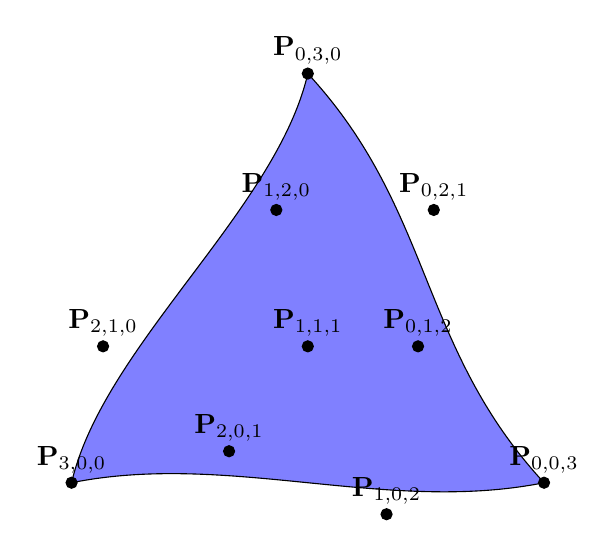
\begin{tikzpicture}[every node/.style={black}]
%	\coordinate (    ) at (Y+Z*2    , Y*1.7320508075    );
\coordinate (p300) at (0+0*2    , 0*1.7320508075    );
\coordinate (p210) at (1+0*2-0.6, 1*1.7320508075    );
\coordinate (p201) at (0+1*2    , 0*1.7320508075+0.4);
\coordinate (p120) at (2+0*2+0.6, 2*1.7320508075    );
\coordinate (p111) at (1+1*2    , 1*1.7320508075    );
\coordinate (p102) at (0+2*2    , 0*1.7320508075-0.4);
\coordinate (p030) at (3+0*2    , 3*1.7320508075    );
\coordinate (p021) at (2+1*2+0.6, 2*1.7320508075    );
\coordinate (p012) at (1+2*2-0.6, 1*1.7320508075    );
\coordinate (p003) at (0+3*2    , 0*1.7320508075    );
\coordinate (p300) at (0+0*2    , 0*1.7320508075    );

\filldraw[fill=blue!50] (p300) .. controls (p210) and (p120) ..  (p030) .. controls (p021) and (p012) .. (p003) .. controls (p102) and (p201) .. (p300);

\filldraw (p300) node[above]{$\mathbf{P}_{3,0,0}$} circle(2pt);
\filldraw (p210) node[above]{$\mathbf{P}_{2,1,0}$} circle(2pt);
\filldraw (p201) node[above]{$\mathbf{P}_{2,0,1}$} circle(2pt);
\filldraw (p120) node[above]{$\mathbf{P}_{1,2,0}$} circle(2pt);
\filldraw (p111) node[above]{$\mathbf{P}_{1,1,1}$} circle(2pt);
\filldraw (p102) node[above]{$\mathbf{P}_{1,0,2}$} circle(2pt);
\filldraw (p030) node[above]{$\mathbf{P}_{0,3,0}$} circle(2pt);
\filldraw (p021) node[above]{$\mathbf{P}_{0,2,1}$} circle(2pt);
\filldraw (p012) node[above]{$\mathbf{P}_{0,1,2}$} circle(2pt);
\filldraw (p003) node[above]{$\mathbf{P}_{0,0,3}$} circle(2pt);

\end{tikzpicture}

An example Cubic Bézier Triangle with control points shown.
\end{center}

% Copyright 2024 Kieran W Harvie. All rights reserved.

\section{Comparison}
\[\begin{array}{|c|c|c|c|}
	\hline
	&Points& Parameters & Mixing\\
	\hline
	Curve&\begin{matrix} A&B \end{matrix}& t_0+t_1=1& At_0+Bt_1\\
		\hline
	Rectangle&\begin{matrix} A&B\\C&D \end{matrix}& t_0+t_1=\tau_0+\tau_1=1 &At_0\tau_0+Bt_1\tau_1+Ct_0\tau_0+Dt_1\tau_1\\
		\hline
	Triangle&\begin{matrix} A&B\\\multicolumn{2}{c}{C} \end{matrix}& t_0+t_1+t_2=1 &At_0+Bt_1+Ct_2\\
		\hline
\end{array}\]
History, 
redundancy,
degeneracy,
and notation convention.


\chapter{Blossom Theory}
% Copyright 2024 Kieran W Harvie. All rights reserved.

Consider a function $f:N\rightarrow M$ where $N$ and $M$ are $R$-modules over a commutative ring $R$\footnote{
We will also use the common convention that,
when it would be useful and wouldn't cause confusion (such as when $N=R$),
Gibbs notation will be dropped.
}.
A blossom $\mathcal{B}[f]$ is a $n$-variate function with the following properties:
\begin{itemize}
	\item {\bf Symmetric in Arguments:} For all $i\leq j\leq n$ we have:
		\[\mathcal{B}[f](\mathbf{t}_1,\cdots, \mathbf{t}_i, \cdots, \mathbf{t}_j, \cdots, \mathbf{t}_n) 
		= \mathcal{B}[f](\mathbf{t}_1,\cdots, \mathbf{t}_j, \cdots, \mathbf{t}_i, \cdots, \mathbf{t}_n) \]
	\item {\bf Affine:} For all $\sum_kw_k=1$ we have:
		\[\mathcal{B}[f]\left(\sum_kw_k\mathbf{s}_k,\mathbf{t}_2,\cdots,\mathbf{t}_n\right) = \sum_kw_k\mathcal{B}[f](\mathbf{s}_k,\mathbf{t}_2,\cdots,\mathbf{t}_n)\]
		Note that affinity combined with symmetry means $\mathcal{B}[f]$ would be affine in all arguments,
		this property is called multi-affine.
	\item {\bf Diagonal:} For all $\mathbf{t}$ we recover:
		\[\mathcal{B}[f](\mathbf{t},\mathbf{t},\cdots,\mathbf{t}) = f(\mathbf{t})\]
\end{itemize}
It will turn out that in practice the strucuture of $M$ isn't that important to blossom theory is overshadowed by the $n$-variance of $f$ and $N$, in particular the dimension of $N$ if appropriate.

% Copyright 2024 Kieran W Harvie. All rights reserved.

\section{Blossom of a Quadratic Bézier Curve}
Consider the function $f:\mathbb{R}\rightarrow\mathbb{R}^m$ used to define the  Quadratic Bézier curve with control points $\{P_0,P_1,P_2\}$:
\[f(t)=(1-t)^2P_0+2t(1-t)P_1+t^2P_2\]
It has the following bivariate blossom:
\[\mathcal{B}[f](t_1,t_2) = (1-t_1)(1-t_2)P_0+((1-t_1)t_2+(1-t_2)t_1)P_1+t_1t_2P_2\]
$\mathcal{B}[f]$ is the archetypal blossom,
Bézier Curves are the context blossoms where made to tackle,
and it having argument symmetry and diagonality can be verified by inspection.
And affinity follows by coefficient-wise substitution, for example:
\[\begin{aligned}
	w_0(1-s_0)+w_1(1-s_1)=& w_0+w_1-(w_0s_0+w_1s_1)\\
	=&1-(w_0s_0+w_1s_1)\\
\end{aligned}\]
Observe that we reclaim the original control points when $(t_1,t_2)\in\{0,1\}^2$:
\[
	f(0,0) = P_1\quad
	f(0,1) = P_2\quad
	f(1,1) = P_3
\]
Also observe that the sum of all the coefficients is $1$:
\[(1-s)(1-t)+((1-s)t+(1-t)s)+st = 1\]
This means the tuple can be interpreted as \hyperref[appx:bary]{barycentric coordinates} of the curve:
\[\big((1-s)(1-t),(1-s)t+(1-t)s,st\big)\]


% Copyright 2024 Kieran W Harvie. All rights reserved.

\section{Structure of $N$}
There are a lot of important results about how the structure of $N$ effects blossoms.

\subsubsection{$N$ has a basis:}
Let $N$ have the basis $\{\mathbf{b}_k\}_k$ and consider and following expansion of an argument $\mathbf{t}_1$:
\[\mathbf{t}_1 = \sum_kr_k\mathbf{b}_k = \sum_kr_k\mathbf{b}_k + \left(1-\sum_rr_k\right)\mathbf{0}\]
Applying affinity we get:
\[\mathcal{B}[f](\mathbf{t}_1,\cdots,\mathbf{t}_n) = \sum_kr_k\mathcal{B}[f](\mathbf{b}_k,\cdots,\mathbf{t}_n)+\left(1-\sum_kr_k\right)\mathcal{B}[f](\mathbf{0},\cdots,\mathbf{t}_n) \]
Iteratively applying this to all arguments we can see that a blossom is fully defined by its values when all the arguments are basis element or $\mathbf{0}$.
Because of this convenient to talk of the control points of a blossom instead of a function, that is we define the function on this set and then get the blossom and function from working backwards.
\\

Consider the case $\dim(N)=1$,
alongside making $N=R$ it lets use the standard indicator function trick to write the previous result as:
\[\begin{aligned}
	\mathcal{B}[f](t_1,t_2,\cdots,t_n) 
	= t_1\mathcal{B}[f](1,t_2,\cdots,t_n)+(1-t_1)\mathcal{B}[f](0,t_2,\cdots,t_n)\\
	= \sum_{\tau_1 \in \{0,1\}}\mathcal{B}[f](\tau_11,t_2,\cdots,t_n)((1-t_1)(1-\tau_1)+t_1\tau_1)\\
\end{aligned}\]
Iteratively do this for all arguments to obtain:
\[\mathcal{B}[f](t_1,t_2,\cdots, t_n) = \sum_{(\tau_k)_{k=0}^n\in\{0,1\}^n}\mathcal{B}[f](\tau_1,\tau_2,\cdots, \tau_n)\prod_{k=1}^n\big((1-t_k)(1-\tau_k)+t_k\tau_k\big)\]
If we $\mathcal{B}[f]_k$
Now consider diagonally to get:
\[f(t) = \mathcal{B}[f](t,t,\cdots,t) = \sum_{k=0}^n\binom{n}{k}t^{n-k}(1-t)^k\mathcal{B}[f]_k\]

% Kept in case I wish to restore the use of boldface.
% 
% Consider the case $\dim(N)=1$;,kj
% In this case there is a single basis element $\mathbf{1}$ and all elements $\mathbf{t}_n$ can be written as:
% \[\mathbf{t}_n = t_n\mathbf{1} \text{ for some } t_n\in R\]
% Applying affinity we get:
% \[\begin{aligned}
% 	\mathcal{B}[f](\mathbf{t}_1,\mathbf{t}_2,\cdots,\mathbf{t}_n) 
% 	= t_1\mathcal{B}[f](\mathbf{1},\mathbf{t}_2,\cdots,\mathbf{t}_n)+(1-t_1)\mathcal{B}[f](\mathbf{0},\mathbf{t}_2,\cdots,\mathbf{t}_n)\\
% 	= \sum_{\tau_1 \in \{0,1\}}\mathcal{B}[f](\tau_1\mathbf{1},\mathbf{t}_2,\cdots,\mathbf{t}_n)((1-t_1)(1-\tau_1)+t_1\tau_1)\\
% \end{aligned}\]
% We can iteratively do this for all arguments to obtain:
% \[\mathcal{B}[f](\mathbf{t}_1,\mathbf{t}_2,\cdots, \mathbf{t}_n) = \sum_{(\tau_k)_{k=0}^n\in\{0,1\}^n}\mathcal{B}[f](\tau_1\mathbf{1},\tau_2\mathbf{1},\cdots, \tau_n\mathbf{1})\prod_{k=1}^n\big((1-t_k)(1-\tau_k)+t_k\tau_k\big)\]

\subsubsection{Field and coordinates, bases, and the matrix}

\subsubsection{Example: $N=\mathbb{R}^n,M=\mathbb{R}^m,$ and $R=\mathbb{R}$}
While there are a lot of interesting properties of general blossoms\footnote{For example, the Bernstein polynomials are useful for uniformly approximating any continuous function and this property carries to blossoms.},
for the rest of this document we will be considering blossoms where the values $\mathcal{B}[f]_k$ are fixed points in $\mathbb{R}^m$ and then defining $f$ through the previous formula.
From the previous result this approach is valid when we make $f$ have a number of arguments greater than or equal to the number of points minus one.

Explicitly,we define $b$ to be the blossom over the points $P_k$
Because the function $f$ has been so heavily demoted 
\[b(t_1,t_2,\cdots,t_n) = \mathcal{B}[f](t_1,t_2,\cdots,t_n)\]

\subsubsection{Example: $f$ is a polynomial}
Observe that the coefficients are Bernstein polynomials of degree $n$.
These polynomials are known to form a basis of polynomials of degree $n$ or less.
Hence when $f$ is a polynomial of degree $n$ the blossom $\mathcal{B}[f]$ is uniquely defined when it is $n$-variate or greater and we can calculate $\mathcal{B}[f]$ by setting $\mathcal{B}[f]_k$ to the coefficients of $f$ in the Bernstein basis.


% Copyright 2024 Kieran W Harvie. All rights reserved.

\section{Blossom of a Cubic Bézier Triangle}
Consider the function $f:\mathbb{R}^3\rightarrow\mathbb{R}^m$ that's used to define the  Cubic Bézier triangle:
\[\begin{aligned}
	f(\lambda_0,\lambda_1,\lambda_2) =& \lambda_0^3P_{0,0,0}+\lambda_1^3P_{1,1,1}+\lambda_2^3P_{2,2,2}\\
	&+3\lambda_0^2\lambda_1P_{0,0,1}+3\lambda_0^2\lambda_2P_{0,0,2}\\
	&+3\lambda_1^2\lambda_0P_{0,1,1}+3\lambda_1^2\lambda_2P_{1,1,2}\\
	&+3\lambda_2^2\lambda_0P_{0,2,2}+3\lambda_2^2\lambda_1P_{1,2,2}\\
	&+6\lambda_0\lambda_1\lambda_2P_{0,1,2}\\
\end{aligned}\]
It has the following 
\[\begin{aligned}
	&\mathcal{B}[f]((\lambda_{0,0},\lambda_{0,1},\lambda_{0,2}),(\lambda_{1,0},\lambda_{1,1},\lambda_{1,2}),(\lambda_{2,0},\lambda_{2,1},\lambda_{2,2}))\\
	=&P_{0,0,0}\lambda_{0, 0} \lambda_{1, 0} \lambda_{2, 0}
	+P_{1,1,1} \lambda_{0, 1} \lambda_{1, 1} \lambda_{2, 1}
	+P_{2,2,2} \lambda_{0, 2} \lambda_{1, 2} \lambda_{2, 2}\\
	&+P_{0,0,1} (\lambda_{0, 1} \lambda_{1, 0} \lambda_{2, 0} + \lambda_{0, 0} \lambda_{1, 1} \lambda_{2, 0} + \lambda_{0, 0} \lambda_{1, 0} \lambda_{2, 1})\\
	&+P_{0,0,2} (\lambda_{0, 2} \lambda_{1, 0} \lambda_{2, 0} + \lambda_{0, 0} \lambda_{1, 2} \lambda_{2, 0} + \lambda_{0, 0} \lambda_{1, 0} \lambda_{2, 2})\\
	&+P_{0,1,1} (\lambda_{0, 1} \lambda_{1, 1} \lambda_{2, 0} + \lambda_{0, 1} \lambda_{1, 0} \lambda_{2, 1} + \lambda_{0, 0} \lambda_{1, 1} \lambda_{2, 1})\\
	&+P_{0,2,2} (\lambda_{0, 2} \lambda_{1, 2} \lambda_{2, 0} + \lambda_{0, 2} \lambda_{1, 0} \lambda_{2, 2} + \lambda_{0, 0} \lambda_{1, 2} \lambda_{2, 2})\\
	&+P_{1,1,2} (\lambda_{0, 2} \lambda_{1, 1} \lambda_{2, 1} + \lambda_{0, 1} \lambda_{1, 2} \lambda_{2, 1} + \lambda_{0, 1} \lambda_{1, 1} \lambda_{2, 2})\\
	&+P_{1,2,2} (\lambda_{0, 2} \lambda_{1, 2} \lambda_{2, 1} + \lambda_{0, 2} \lambda_{1, 1} \lambda_{2, 2} + \lambda_{0, 1} \lambda_{1, 2} \lambda_{2, 2})\\
	&+P_{0,1,2} (\lambda_{0, 2} \lambda_{1, 1} \lambda_{2, 0} + \lambda_{0, 1} \lambda_{1, 2} \lambda_{2, 0} + \lambda_{0, 2} \lambda_{1, 0} \lambda_{2, 1}\\
	&\quad+ \lambda_{0, 0} \lambda_{1, 2} \lambda_{2, 1} + \lambda_{0, 1} \lambda_{1, 0} \lambda_{2, 2} + \lambda_{0, 0} \lambda_{1, 1} \lambda_{2, 2})\\
\end{aligned}\]



\chapter{The Blossoming}
% Copyright 2024 Kieran W Harvie. All rights reserved.

The main computational use for blossoms is called "The Blossoming" and is a way to calculate to caclulate the blossom for arbitary values.
The input is all combination from 
intermidite values in the calculation will also be useful
Main recursive function
two main contrants the dimenion of $N$ and the $n$-variance of the function
\[\binom{n}{\dim(N)}\]
Like the previous is 

% Copyright 2024 Kieran W Harvie. All rights reserved.

\section{The Blossoming of a Cubic Bézier Curve}
Let $b$ 
\[\begin{matrix}
	&t_1&t_2&t_3\\
	\hline
	\mathcal{B}[f](a,a,a)&\mathcal{B}[f](a,a,t_1)&\mathcal{B}[f](a,t_2,t_1)&\mathcal{B}[f](t_3,t_2,t_1)\\
	\mathcal{B}[f](a,a,b)&\mathcal{B}[f](a,b,t_1)&\mathcal{B}[f](b,t_2,t_1)&\\
	\mathcal{B}[f](a,b,b)&\mathcal{B}[f](b,b,t_1)&&\\
	\mathcal{B}[f](b,b,b)&&&\\
\end{matrix}\]
\[\mathcal{B}[f](a,a,t_k) = \frac{b-t_k}{b-a}\mathcal{B}[f](a,a,a)+\frac{t_k-a}{b-a}\mathcal{B}[f](a,a,b)\]

% Copyright 2024 Kieran W Harvie. All rights reserved.

\section{The Blossoming of a Cubic Bézier Triangle}
We take $F=\mathbb{R}$, $N=\mathbb{R}^2$, and $M=\mathbb{R}^m$
comonly $m$ is $2$ or $3$.
\begin{center}
\begin{tikzpicture}[every node/.style={black}]
	\coordinate (e0) at (0,0);
	\coordinate (e1) at (4*0.5,4*0.86602540378);
	\coordinate (e2) at (4,0);

	\draw[-stealth] (e0)--(e1);
	\draw[-stealth] (e0)--(e2);

	\filldraw (e0) node[left]{$\mathbf{e}_0=\mathbf{0}$} circle(2pt);
	\filldraw (e1) node[above]{$\mathbf{e}_1=\mathbf{b}_1$} circle(2pt);
	\filldraw (e2) node[right]{$\mathbf{e}_2=\mathbf{b}_2$} circle(2pt);
\end{tikzpicture}
\end{center}

Cubic case
\[\mathbf{t} = \lambda_0\mathbf{e}_0+\lambda_1\mathbf{e}_1+\lambda_2\mathbf{e}_2\]
\[b(\mathbf{t}) = \lambda_0b(\mathbf{e}_0)+\lambda_1b(\mathbf{e}_1)+\lambda_2b(\mathbf{e}_2)\]
\[\begin{aligned}
	b(\mathbf{t},\mathbf{t})=& \lambda_0^2b(\mathbf{e}_0,\mathbf{e}_0)+\lambda_1^2b(\mathbf{e}_1,\mathbf{e}_1)+\lambda_2^2b(\mathbf{e}_2,\mathbf{e}_2)\\
	&+2\lambda_0\lambda_1b(\mathbf{e}_0,\mathbf{e}_1)+2\lambda_1\lambda_2b(\mathbf{e}_1,\mathbf{e}_2)+2\lambda_1\lambda_2b(\mathbf{e}_1,\mathbf{e}_2)
\end{aligned}\]

each argument can have a different $\mathbf{t}$

\begin{center}
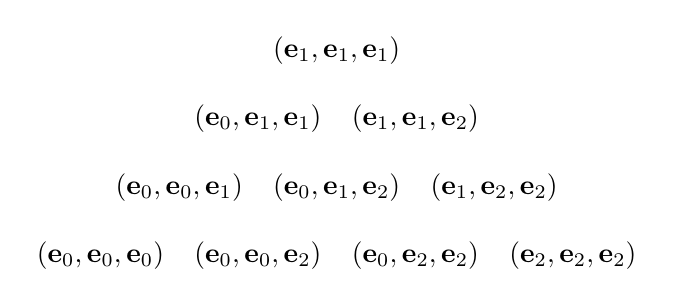
\begin{tikzpicture}[every node/.style={black}]
%	\coordinate (    ) at (Y+Z*2    , Y*1.7320508075    );
	\coordinate (e000) at (0+0*2, 0*0.86602540378);
	\coordinate (e001) at (1+0*2, 1*0.86602540378);
	\coordinate (e002) at (0+1*2, 0*0.86602540378);
	\coordinate (e011) at (2+0*2, 2*0.86602540378);
	\coordinate (e012) at (1+1*2, 1*0.86602540378);
	\coordinate (e022) at (0+2*2, 0*0.86602540378);
	\coordinate (e112) at (2+1*2, 2*0.86602540378);
	\coordinate (e122) at (1+2*2, 1*0.86602540378);
	\coordinate (e222) at (0+3*2, 0*0.86602540378);
	\coordinate (e111) at (3+0*2, 3*0.86602540378);

	\filldraw (e000) node{$(\mathbf{e}_0,\mathbf{e}_0,\mathbf{e}_0)$};
	\filldraw (e001) node{$(\mathbf{e}_0,\mathbf{e}_0,\mathbf{e}_1)$};
	\filldraw (e011) node{$(\mathbf{e}_0,\mathbf{e}_1,\mathbf{e}_1)$};
	\filldraw (e002) node{$(\mathbf{e}_0,\mathbf{e}_0,\mathbf{e}_2)$};
	\filldraw (e012) node{$(\mathbf{e}_0,\mathbf{e}_1,\mathbf{e}_2)$};
	\filldraw (e111) node{$(\mathbf{e}_1,\mathbf{e}_1,\mathbf{e}_1)$};
	\filldraw (e022) node{$(\mathbf{e}_0,\mathbf{e}_2,\mathbf{e}_2)$};
	\filldraw (e112) node{$(\mathbf{e}_1,\mathbf{e}_1,\mathbf{e}_2)$};
	\filldraw (e122) node{$(\mathbf{e}_1,\mathbf{e}_2,\mathbf{e}_2)$};
	\filldraw (e222) node{($\mathbf{e}_2,\mathbf{e}_2,\mathbf{e}_2)$};
\end{tikzpicture}\quad\begin{tikzpicture}[every node/.style={black}]
	\filldraw (e001) node{$(\mathbf{e}_0,\mathbf{e}_0,\mathbf{t})$};
	\filldraw (e011) node{$(\mathbf{e}_0,\mathbf{e}_1,\mathbf{t})$};
	\filldraw (e012) node{$(\mathbf{e}_0,\mathbf{e}_2,\mathbf{t})$};
	\filldraw (e111) node{$(\mathbf{e}_1,\mathbf{e}_1,\mathbf{t})$};
	\filldraw (e112) node{$(\mathbf{e}_1,\mathbf{e}_2,\mathbf{t})$};
	\filldraw (e122) node{$(\mathbf{e}_2,\mathbf{e}_2,\mathbf{t})$};
\end{tikzpicture}
\end{center}

\[\begin{aligned}
	b(\mathbf{t},\mathbf{t},\mathbf{t})=& \lambda_0^3b(\mathbf{e}_0,\mathbf{e}_0,\mathbf{e}_0)+\lambda_1^3b(\mathbf{e}_1,\mathbf{e}_1,\mathbf{e}_1)+\lambda_2^3b(\mathbf{e}_2,\mathbf{e}_2,\mathbf{e}_2)\\
	&+3\lambda_0^2\lambda_1b(\mathbf{e}_0,\mathbf{e}_0,\mathbf{e}_1)+3\lambda_0^2\lambda_2b(\mathbf{e}_0,\mathbf{e}_0,\mathbf{e}_2)\\
	&+3\lambda_1^2\lambda_0b(\mathbf{e}_0,\mathbf{e}_1,\mathbf{e}_1)+3\lambda_1^2\lambda_2b(\mathbf{e}_1,\mathbf{e}_1,\mathbf{e}_2)\\
	&+3\lambda_2^2\lambda_0b(\mathbf{e}_0,\mathbf{e}_2,\mathbf{e}_2)+3\lambda_2^2\lambda_1b(\mathbf{e}_1,\mathbf{e}_2,\mathbf{e}_2)\\
	&+6\lambda_0\lambda_1\lambda_2b(\mathbf{e}_0,\mathbf{e}_1,\mathbf{e}_2)\\
\end{aligned}\]


\chapter{Rendering}
% Copyright 2024 Kieran W Harvie. All rights reserved.

Applications of Bézier Triangles and the blossoming in general is turing control points into useful properties/computation.
Rendering is the archetypal application,
where control points are turned into sufficiently small triangles to be convincingly showen on screen.
but other applications 

% Copyright 2024 Kieran W Harvie. All rights reserved.

\section{Direct}
Naive
tesseltion\cite{khronostessellation}
dynamic tesselation
hardware supported

% Copyright 2024 Kieran W Harvie. All rights reserved.

\section{Subdivision}

% Copyright 2024 Kieran W Harvie. All rights reserved.

\section{Point-Normal Triangle}
A way of turning point-normals into a cubic beziedr triangle\cite{pointnormal}


\renewcommand\thesection{A\arabic{section}}

\chapter{Appendix}
% Copyright 2024 Kieran W Harvie. All rights reserved.

\section{Barycentric Coordinates}
\label{appx:bary}
\begin{center}
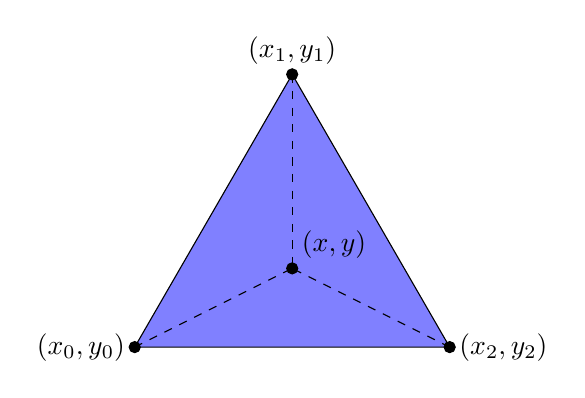
\begin{tikzpicture}[every node/.style={black}]
	\coordinate (p0) at (0,0);
	\coordinate (p1) at (4*0.5,4*0.86602540378);
	\coordinate (p2) at (4,0);
	\coordinate (p) at (2,1);

	\filldraw[fill=blue!50] (p0) -- (p1) -- (p2) -- cycle;

	\draw[dashed] (p0)--(p);
	\draw[dashed] (p1)--(p);
	\draw[dashed] (p2)--(p);

	\filldraw (p0) node[left]{$(x_0,y_0)$} circle(2pt);
	\filldraw (p1) node[above]{$(x_1,y_1)$} circle(2pt);
	\filldraw (p2) node[right]{$(x_2,y_2)$} circle(2pt);
	\filldraw (p) node[above right]{$(x,y)$} circle(2pt);
\end{tikzpicture}
\end{center}
Given three points $(x_n,y_n)$ of a triangle the barycentric coordiates for a point $(x,y)$ are numbers $\lambda_0,\lambda_1,$ and $\lambda_2$ such that:
\[(x,y) = \lambda_0(x_0,y_0)+\lambda_1(x_1,y_1)+\lambda_2(x_2,y_2)\quad \lambda_0+\lambda_1+\lambda_2=1\]
These requirements are equivalent to the following matrix equation:
\[
\begin{bmatrix}
	x_0&x_1&x_2\\
	y_0&y_1&y_2\\
	1&1&1\\
\end{bmatrix}
\begin{bmatrix}
	\lambda_0\\\lambda_1\\\lambda_2\\
\end{bmatrix}
=
\begin{bmatrix}
	x\\y\\1\\
\end{bmatrix}
\]
To analyse this equation start by considering the following identity: 
\[
\begin{vmatrix}
	a_0&a_1&a_2\\
	b_0&b_1&b_2\\
	1&1&1\\
\end{vmatrix}
=
\begin{vmatrix}
	a_0&a_1-a_0&a_2-a_0\\
	b_0&b_1-b_0&b_2-b_0\\
	1&0&0\\
\end{vmatrix}
=
\begin{vmatrix}
	a_1-a_0&a_2-a_0\\
	b_1-b_0&b_2-b_0\\
\end{vmatrix}
\]
This means that the normal requirement for a solution,
that the determinate of the matrix be nonzero,
is equivalent to:
\[
	0\neq
\begin{vmatrix}
	x_0&x_1&x_2\\
	y_0&y_1&y_2\\
	1&1&1\\
\end{vmatrix}
\Leftrightarrow
0\neq
\begin{vmatrix}
	x_1-x_0&x_2-x_0\\
	y_1-y_0&y_2-y_0\\
\end{vmatrix}
\]
It also lets us simplify the solutions for $\lambda_n$ obtained through Cramer's rule:
\[
	\lambda_0 = 
\frac
{\begin{vmatrix}
	x&x_1&x_2\\
	y&y_1&y_2\\
	1&1&1\\
\end{vmatrix}}
{\begin{vmatrix}
	x_0&x_1&x_2\\
	y_0&y_1&y_2\\
	1&1&1\\
\end{vmatrix}}
=
\frac
{\begin{vmatrix}
	x_1-x&x_2-x\\
	y_1-y&y_2-y\\
\end{vmatrix}}
{\begin{vmatrix}
	x_1-x_0&x_2-x_0\\
	y_1-y_0&y_2-y_0\\
\end{vmatrix}}
\]
These results can be interpreted geometrically,
firstly is that a solution exist if and only if the set $\{(x_1-x_0,y_1-y_0),(x_2-x_0,y_2-y_0)\}$ is linearly independent.
Note that this isn't the same as $\{(x_0,y_0),(x_1,y_1),(x_2,y_2)\}$ being linearly independent,
as two points can be on the same line through the origin so long as the third isn't:
\begin{center}
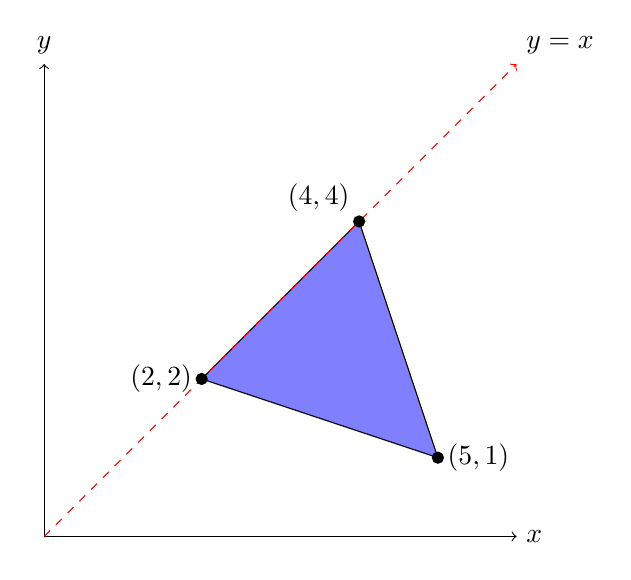
\begin{tikzpicture}[every node/.style={black}]
	\draw[<->] (0,6) node[above]{$y$} -- (0,0) -- (6,0) node[right] {$x$};

	\coordinate (p0) at (2,2);
	\coordinate (p1) at (4,4);
	\coordinate (p2) at (5,1);
	\coordinate (O) at (0,0);

	\filldraw[fill=blue!50] (p0) -- (p1) -- (p2) -- cycle;

	\draw[->, dashed,red] (0,0) -- (6,6) node[above right]{$y=x$};

	\filldraw (p0) node[left]{$(2,2)$} circle(2pt);
	\filldraw (p1) node[above left]{$(4,4)$} circle(2pt);
	\filldraw (p2) node[right]{$(5,1)$} circle(2pt);
\end{tikzpicture}

An example valid triangle with two points lying on the same $y=x$ line.
\end{center}
Secondly is that $\begin{vmatrix}x_1-x&x_2-x\\y_1-y&y_2-y\\\end{vmatrix}$ can be interpreted as the (signed) area of the parallelogram defined by the points $(x_1,y_1)$ and $(x_2,y_2)$ with origin $(x,y)$\footnote{This follows from $\begin{vmatrix}x_1&x_2\\y_1&y_2\\\end{vmatrix}$ being the singed area of the parallelogram of the points $(x_1,y_1)$ and $(x_2,y_2)$ through the origin}.
This means that, 
when $(x,y)$ is contained within the triangle,
$\lambda_0$ can be interpreted as the fraction of the of area the triangle $\{(x,y),(x_1,y_1),(x_2,y_2)\}$ to the area of the larger triangle.
This is why barycentric coordinate are some times called area coordinates. 

\begin{center}
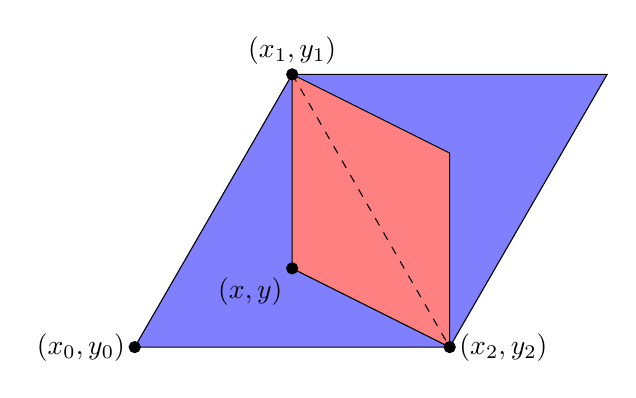
\begin{tikzpicture}[every node/.style={black}]
	\coordinate (p0) at (0,0);
	\coordinate (p1) at (4*0.5,4*0.86602540378);
	\coordinate (p2) at (4,0);
	\coordinate (p3) at (6,4*0.86602540378);
	\coordinate (p) at (2,1);
	\coordinate (r) at (6-2,4*0.86602540378-1);

	\filldraw[fill=blue!50] (p0) -- (p1) -- (p3) -- (p2) --cycle;
	\filldraw[fill=red!50] (p) -- (p1) -- (r) -- (p2) --cycle;

	\filldraw (p0) node[left]{$(x_0,y_0)$} circle(2pt);
	\filldraw (p1) node[above]{$(x_1,y_1)$} circle(2pt);
	\filldraw (p2) node[right]{$(x_2,y_2)$} circle(2pt);
	\filldraw (p) node[below left]{$(x,y)$} circle(2pt);

	\draw[dashed] (p1)--(p2);
\end{tikzpicture}

Visualization of the area properties of barycentric coordinate. 
Observe the shared diagonal that lets us evenly covert the parallelograms to triangles and that the two areas have the same sign.
\end{center}
Finally these arguments can be generalized to other dimensions by making natural modification to the original matrix equation,
three dimensions would give:
\[
\begin{bmatrix}
	x_0&x_1&x_2&x_3\\
	y_0&y_1&y_2&y_3\\
	z_0&z_1&z_2&z_3\\
	1&1&1&1\\
\end{bmatrix}
\begin{bmatrix}
	\lambda_0\\\lambda_1\\\lambda_2\\\lambda_3\\
\end{bmatrix}
=
\begin{bmatrix}
	x\\y\\z\\1\\
\end{bmatrix}
\]
And one would give:
\[
\begin{bmatrix}
	x_0&x_1\\
	1&1\\
\end{bmatrix}
\begin{bmatrix}
	\lambda_0\\\lambda_1\\
\end{bmatrix}
=
\begin{bmatrix}
	x\\1\\
\end{bmatrix}
\]


% Copyright 2024 Kieran W Harvie. All rights reserved.

\section{Notation Variants}
There's two other common notation for the control points of a Bézier Triangle the reader is likely to encounter.

\subsubsection{(Symmetrized) Tensor Product:}
\[(\alpha s + \beta r)^2 = \alpha^2+2\alpha\beta + \beta^2\]
Quadratic Bézier curve:
\[(\lambda_0\mathbf{e}_0+\lambda_1\mathbf{e}_1)^2 = \lambda_0^2\mathbf{e}_0^2+2\lambda_0\lambda_1\mathbf{e}_0\mathbf{e}_1+\lambda_1^2\mathbf{e}_2^2\]
Quadratic Bézier curve blossom:
\[(\lambda_{0,0}\mathbf{e}_0+\lambda_{0,1}\mathbf{e}_1)(\lambda_{1,0}\mathbf{e}_0+\lambda_{1,1}\mathbf{e}_1)\]

Works because of the universal property of the tensor product.
This is probalby the best but like most math it requires a larger upfront cost.
It simplifies and unifies curves and triangles of different orders.

\subsubsection{Weighted}
I think ours links to theory (blossoms) better and this one reflects application better
$P_{i,j,k}$ since they add to $n$ we can see them as weighted 
Particularly when working with Point-Normal triangles.

\subsubsection{Example conversion:}
Still needs to identify corners.
Bloosom 

% I was originally going to include a comparison of the blossoming to the interpolation of a polynomial using the finite difference.
% 
% \section{Finite Difference}
% The finite difference operator $\Delta_h$ is defined as:
% \[\Delta_h[f](x) = f(x+h)-f(x)\]
% We similarly define 
% \begin{equation*}
% \begin{aligned}
% 	\Delta^n_h[f](x) =& \Delta_h[\Delta^{n-1}_h[f]](x)\\
% 	=& \Delta^{n-1}_h[f](x+h)- \Delta^{n-1}_h[f](x)\\
% \end{aligned}
% \end{equation*}
% Let $p_n(x) = x^n$ then:
% \begin{equation*}
% \begin{aligned}
% 	\Delta[p_n](x) =& (x+h)^n-x^n\\
% 	=&\sum_{k=0}^{n-1}\binom{n}{k}h^{n-k}x^k\\
% \end{aligned}
% \end{equation*}


\printbibliography[heading=bibnumbered]

\end{document}
